\section{Controller}
\begin{center}
	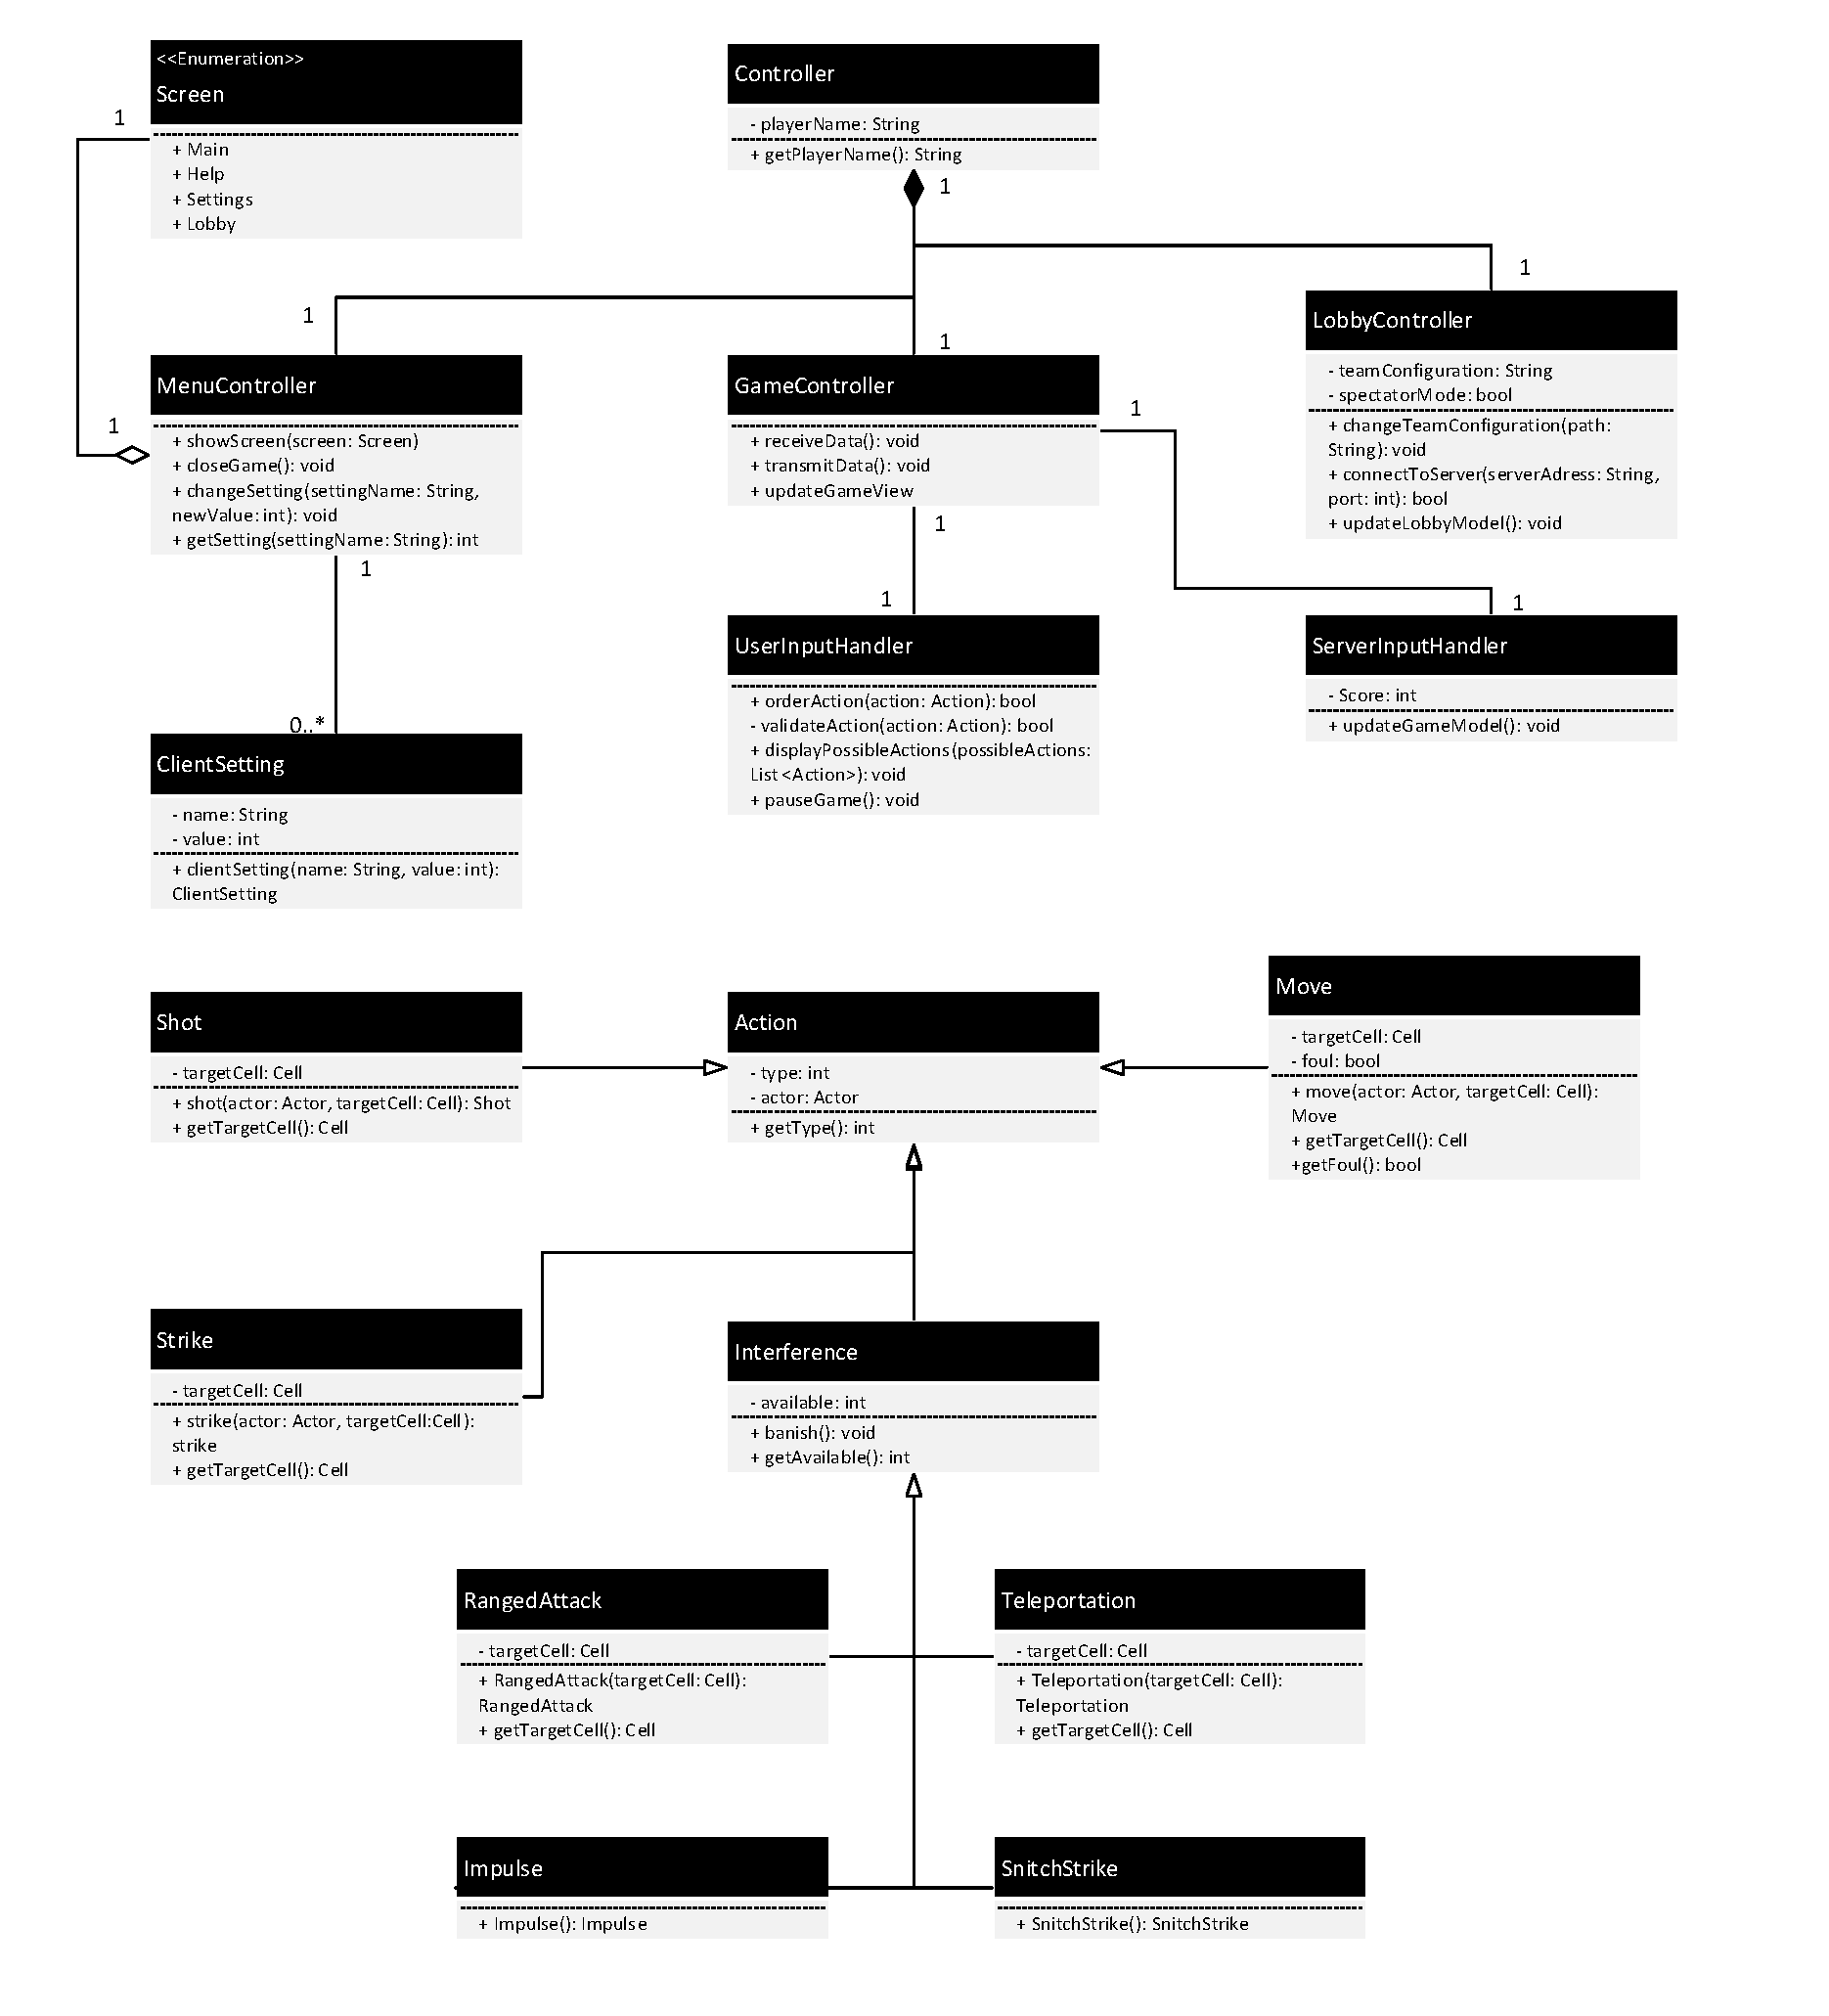
\includegraphics[width=18cm]{images/Klassendiagram_Controller}
\end{center}

	Im Folgenden werden die eingetragenen Methoden erklärt.
\begin{center}
	\begin{tabular}{|p{4.7cm}|p{3.5cm}|p{3.5cm}|p{4.3cm}|}
		\hline
		\textbf{Name} & \textbf{Vorbedingungen} & \textbf{Nachbedingungen} & \textbf{Erklärung}\\\hline
		\multicolumn{4}{|l|}{MenuController} \\\hline
		closeGame & - & Positive Antwort in einem Popup-Fenster & Beendet die Anwendung\\\hline
		changeSetting & ClientSetting mit dem angegebenen settingName existiert & Der Wert von newValue wird akzeptiert & Ändert das Attribut value des ClientSetting mit dem Attribut name, der dem Parameter settingName entspricht, auf den Wert des Parameters newValue.\\\hline
		getSetting& ClientSetting mit dem angegebenen settingName existiert & - & Liefert den derzeitigen Wert des Attributs value des ClientSetting, dessen Attribut name mit dem Parameter settingName übereinstimmt.\\\hline
		\multicolumn{4}{|l|}{GameController} \\\hline
		receiveData & - & - & Empfängt Daten vom JSON-Parser und übergibt sie dem ServerInputHandler\\\hline
		transmitData & - & - & Empfängt Daten vom UserInputHandler und sendet sie über den JSON-Parser und den Kommunikator zum Server\\\hline
		\multicolumn{4}{|l|}{LobbyController} \\\hline
		changeTeamConfiguration & - & Parameter path ist ein gültiger Pfad zu einer Team-Konfigurations-Datei & Ändert den Wert von teamConfiguration, in dem der Pfad zu der zu verwendenden Team-Konfigurations-Datei gespeichert ist.\\\hline
		
	\end{tabular}
	
	\begin{tabular}{|p{4.7cm}|p{3.5cm}|p{3.5cm}|p{4.3cm}|}	
		\hline
		connectToServer & Parameter serverAdress und port sind ungleich Null & - & Veranlasst über den JSON-Parser den Kommunikator dazu, eine Verbindung mit dem in den Parametern spezifiziertem Server aufzubauen. Gibt true zurück, wenn der Verbindungsaufbau erfolgreich war, ansonsten false.\\\hline
		\multicolumn{4}{|l|}{UserInputHandler} \\\hline
		validateAction & - & - & Fordert vom Partie-Model Daten an und entscheidet danach, ob die geforderte Action durchgeführt werden kann. Gibt true zurück wenn die als Parameter übergebene Action gültig ist, ansonsten false.\\\hline
		orderAction & validateAction gibt für die als Parameter übergebene Action true zurück. & - & Übergibt die auszuführende Aktion an den GameController. Ruft die Methode validateAction auf und gibt deren Rückgabewert zurück.\\\hline
		displayPossibleActions & - & - & Fordert vom Partie-Model Daten an und berechnet alle möglichen Aktionen und gibt sie an die Partie-View weiter, um sie dem Spieler anzuzeigen.\\\hline
		\multicolumn{4}{|l|}{Interference} \\\hline
		banish & - & - & Verringert das Attribut available um eins.\\\hline
		
	\end{tabular}
\end{center}

Die Funktionalen Anforderungen werden den Methoden folgendermaßen zugeteilt:
\begin{center}
	\begin{tabular}{|l|l|}
		\hline
		\textbf{Funktionale Anforderungen} & \textbf{Methoden}\\\hline
		FA7 & Shot::shot\\
		& Shot::getTargetCell\\\hline
		FA21 & Shot::shot\\\hline
		FA26 & Move::move\\\hline
		FA27 & Shot::shot\\\hline
		FA28 & Strike::strike\\\hline
		FA30 & Move::move\\\hline
		FA31 & RangedAttack::rangedAttack\\
		& Teleportation::teleportation\\
		& Impulse::impulse\\
		& SnitchStrike::snitchStrike\\
		& Inteference::banish\\\hline
		FA32 & Teleportation::teleportation\\\hline
		FA33 & RangedAttack::rangedAttack\\\hline
		FA34 & Impulse::impulse\\\hline
		FA35 & SnitchStrike::snitchStrike\\\hline
		FA36 & Inteference::banish\\
		& Actor::setBanished\\\hline
		FA37 & Actor::setBanished\\
		& Move::move\\\hline
		FA38 - FA42 & Move::move\\\hline
		FA48 & Actor::setBanished\\\hline
		FA54 & LobbyController::changeTeamConfiguration\\
		& LobbyController::updateLobbyModel\\\hline
		FA55 & GameController::receiveData\\
		& GameController::transmitData\\
		& LobbyController::connectToServer\\\hline
		FA56 & GameController::receiveData\\
		& GameController::transmitData\\\hline
		FA60-FA61 & MenuController::showScreen\\\hline
		FA67 & UserInputHandler::orderActions\\
		& UserInputHandler::validateActions\\
		& MenuController::showScreen\\
		& MenuController::changeSetting\\
		& LobbyController::changeTeamConfiguration\\
		& LobbyController::connectToServer\\\hline
		FA69 & UserInputHandler::pauseGame\\\hline
		
	\end{tabular}
\end{center}
